\documentclass{article}
\usepackage{hyperref}
\usepackage{graphicx}

\begin{document}

\title{Pinkdev\\
SDK for Image Processing Operators
}
\author{M. Couprie and L. Najman}

\maketitle
\section{Introduction}

This environment aims at facilitating the development of your first
image processing operators. It includes features such as input/output
that allows reading and writing grey-scale images, under the {\bf pgm}
format.  pgm stands for Portable Gray Map, and this is the name of a
standard format. Pinkdev also proposes a data structure allowing to
manipulate image pixels, once an image is loaded into memory.

To visualize images, any standard tool can be used. We recommand {\bf
  imview}, but are not sure it is available everywhere at ESIEE.  You
can install it at home, following this link
\url{http://hugues.zahlt.info/Imview.html}.


\section{xvimage structure}

An image is seen as a rectangular table, with two dimensions of {\em
  pixels} or picture elements. The intensity of each pixel (its grey
level) es thus given by a byte (unsigned char, value between 0 and
255).

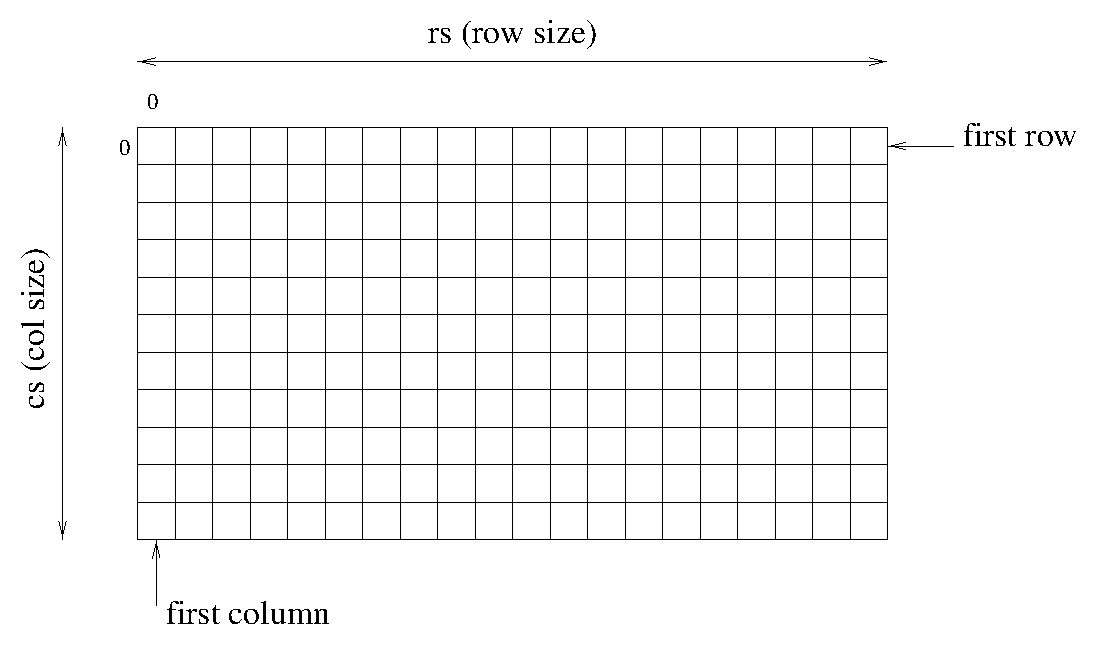
\includegraphics{xvimage1}

In memory, an image is stored in a structure of type {\bf xvimage}:

\begin{verbatim}
struct xvimage {
  char *name;
  uint32_t row_size;                    /* Size of a row (number of columns) */
  uint32_t col_size;                    /* Size of a column (number of rows) */
  uint32_t depth_size;                  /* Number of planes (for 3d images) */
  uint32_t data_storage_type;           /* storage type for disk data */
  void * image_data;                    /* pointer on raw data */
};
\end{verbatim}

While using this structure, the array {\bf imagedata} is a one
dimensional array whose size depends on the size of the image to
store. If the image is of size $m\times n$, then {\bf imagedata} is of
size $mn$. Pixels are stored in this array in the following order.

\begin{verbatim}
pixel 0 of line 1
pixel 1 of line  1
...
pixel row_size-1 of line  1
pixel 0 of line 2
...
\end{verbatim}

\section{Accessing a pixel}


To access a pixel we first need to get the address of the array that
contains the pixels:
\begin{verbatim}
  ptrimage = (unsigned char *)(image->imagedata);
\end{verbatim}

Then, to access the $i^{\mbox{th}}$ pixel of the $j^{\mbox{th}}$ row,
we can use the following:

\begin{verbatim}
  ptrimage[j * rs + i]
\end{verbatim}

\section{An example}

Here is an example of a {\bf laddconst} function that add a constant
value to the greyscale value of each pixel, unless such an operation
will overflow 255. The source code is located in:
\verb|src/lib/laddconst.c|, the header file is:
\verb|include/laddconst.h|:

\begin{verbatim}
/* ajoute une constante a une image  - seuil si depassement */
/* Add a const to an image - thresholding if overflow */
/* Michel Couprie - janvier 1999 */

#include <stdio.h>
#include <stdlib.h>
#include <laddconst.h>
#include <mcimage.h>

/* ==================================== */
int laddconst(struct xvimage * image, /* input: image to process */
                                      /* output: modified image  */
              int constante           /* input: value to add */
             )
/* ==================================== */
{
  int indexpixel;
  unsigned char *ptrimage;
  unsigned long newval;
  int rs, cs, N;

  rs = image->row_size;
  cs = image->col_size;
  N = rs * cs;
  
  /* ---------------------------------------------------------- */
  /* computing the result */
  /* ---------------------------------------------------------- */
  ptrimage = (unsigned char *)(image->imagedata);
  for (indexpixel = 0; indexpixel < N; indexpixel++)
  {
    newval = (int)(ptrimage[indexpixel]) + constante;
    if (newval < NDG_MIN) newval = NDG_MIN;
    if (newval > NDG_MAX) newval = NDG_MAX;
    ptrimage[indexpixel] = (unsigned char)newval;
  }

  return 1; /* Everything went fine */
}
\end{verbatim}

Of course, we need a main to compile this fucntion. The main has to do
the three following operations: to read the image from a file, to call
the {\bf laddconst} function, and to store the result in another file.

\section{Reading image files}

Reading an image from a file with the pgm format is dont thanks to a
call to the function {\bf readimage}:

\begin{verbatim}
  struct xvimage * image;
  char *filename;
  ...
  image = readimage(filename);  
\end{verbatim}

This function returns a NULL pointer if the reading did not run
correctly. The function {\bf readimage} is defined in
\verb|src/lib/mcimage.c|, while the header is in
\verb|include/mcimage.h|.


\section{Writing an image file}

Writing an image in the {\bf pgm} format is done thanks to a call to
the function {\bf writeimage}:

\begin{verbatim}
  struct xvimage * image;
  char *filename;
  ...
  writeimage(image, filename);
\end{verbatim}

The function {\bf writeimage} is defined in \verb|src/lib/mcimage.c|,
while the header is in \verb|include/mcimage.h|.

\section{Allocating a structure {\bf xvimage}}

In a call to {\bf readimage}, a {\bf xvimage} structure is
automatically allocated. To allocate an {\bf xvimage} structure
without a call to {\bf readimage}, we can use the function {\bf
  allocimage}:

\begin{verbatim}
  struct xvimage * image;
  int rs, cs;
  ...  
  image = allocimage(NULL, rs, cs, 1, VFF_TYP_1_BYTE);
\end{verbatim}

To free the allocated memory, we can use the function
{\bf freeimage}:

\begin{verbatim}
  freeimage(image);
\end{verbatim}

The functions {\bf allocimage} and {\bf freeimage} are defined in
\verb|src/lib/mcimage.c|, while the headers are in
\verb|include/mcimage.h|.

\section{An example}
Here is a main that calls the function
{\bf laddconst} (source: \verb|src/com/addconst.c|):

\begin{verbatim}
/* Call to laddconst */

#include <stdio.h>
#include <mcimage.h>
#include <laddconst.h>

/* =============================================================== */
int main(int argc, char **argv) 
/* =============================================================== */
{
  struct xvimage * image1;
  int constante;

  if (argc != 4)
  {
    fprintf(stderr, "usage: %s in1.pgm constante out.pgm \n", argv[0]);
    exit(0);
  }

  image1 = readimage(argv[1]);  
  if (image1 == NULL)
  {
    fprintf(stderr, "addconst: readimage failed\n");
    exit(0);
  }
  constante = atoi(argv[2]);

  if (! laddconst(image1, constante))
  {
    fprintf(stderr, "addconst: function laddconst failed\n");
    exit(0);
  }

  writeimage(image1, argv[3]);
  freeimage(image1);

} /* main */
\end{verbatim}

\section{Directories}

doc      : documentation\\
include  : header files (.h)\\
obj      : object files (.o)\\
bin      : executables\\
src/com  : sources of the programs that will be run from shell\\
src/lib  : sources of the basic (mcimage) and processing functions

\end{document}
